\documentclass[../../main]{subfiles}
\begin{document}

\subsection{Points of Interest}
\label{ss:final-poi}

A point of interest, as described earlier, is a collection of data like position, category and name that are rapresented on the map as a marker of 
different colour based on the category. A user can create a poi touching the map or by inserting an address (actually disabled because the api is not free),
 delete it and also sharing it by an url for google maps.
In the next picture we can see the list of poi and the dialog to create it.
\begin{figure}[H]
    \centering
    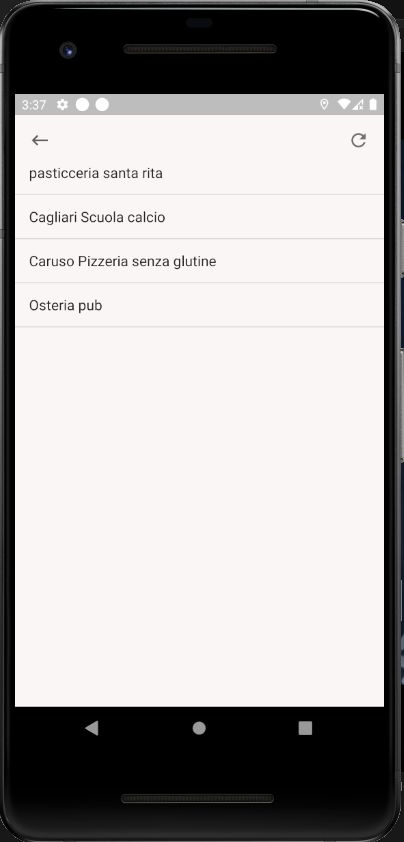
\includegraphics[width=70mm,height=150mm]{images/app/poi/poi_overview.png}
    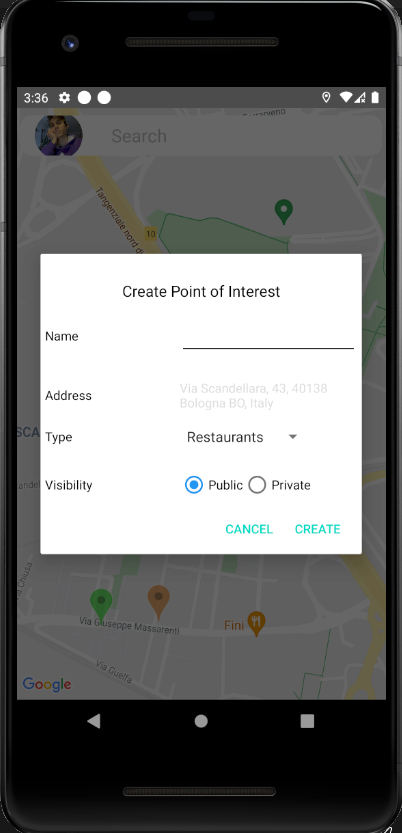
\includegraphics[width=70mm,height=150mm]{images/app/poi/creazione_poi.png}
    \caption{On the left the overview of the pois list and on the right the dialog to create a poi.}
\end{figure}
By clicking on a poi is possible to see its detail and to share it as mentioned before.

\begin{figure}[H]
    \centering
    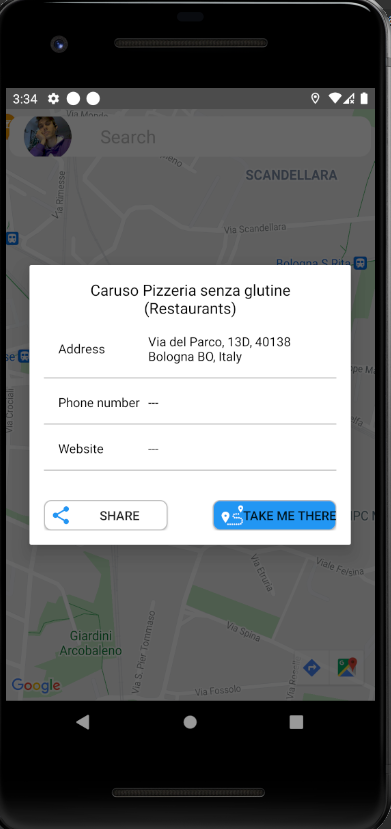
\includegraphics[width=70mm,height=150mm]{images/app/poi/poi_map_detail.png}
    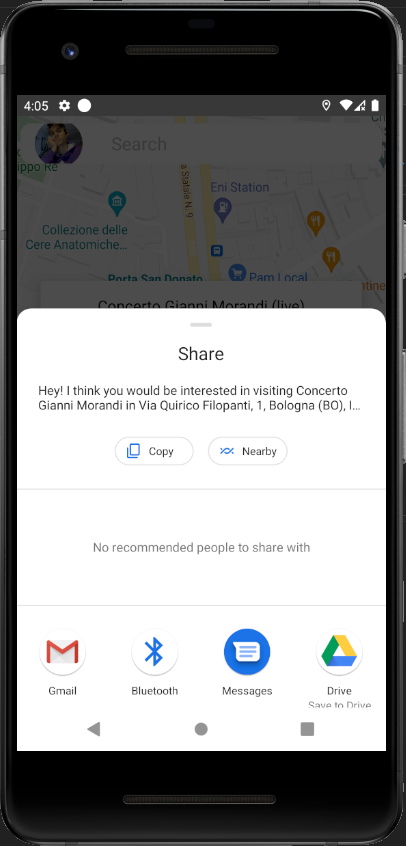
\includegraphics[width=70mm,height=150mm]{images/app/share.png}
    \caption{On the left the dialog to look at the detail of a poi and on the right the sharing of a poi url.}
\end{figure}
\end{document}